\chapter{IMPLEMENTAÇÃO}

O modelo proposto é uma arquitetura de \textbf{Rede Neural Artificial Profunda} com dados heterogêneos não estruturados. Seu formato é a combinação de outras arquiteturas já conhecidas e amplamente utilizadas para resolver separadamente problemas de \textbf{Processamento de Linguagem Natural} e \textbf{Visão Computacional}.

\begin{figure}[!h]
	\caption{\label{arquitetura_macro_do_modelo} Arquitetura Macro do Modelo}
	\begin{center}
	    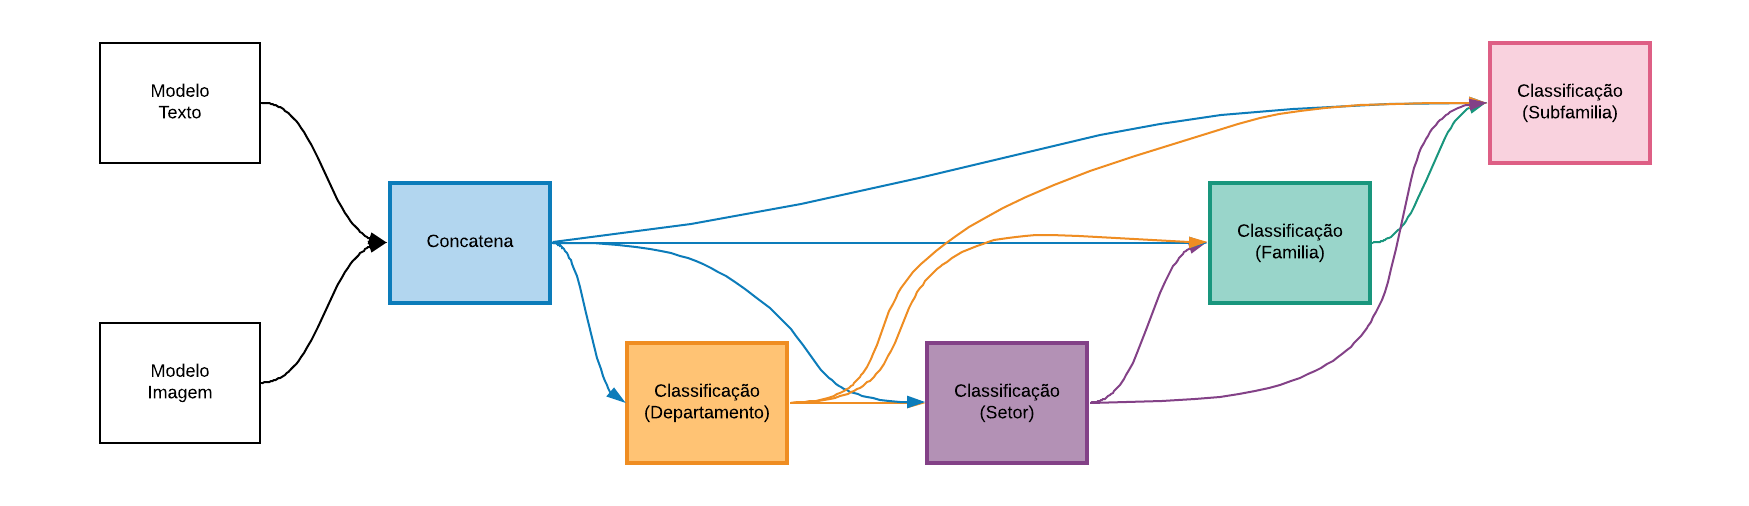
\includegraphics[width=\textwidth]{artigo/recursos/imagens/arquitetura_macro_do_modelo.png}
	\end{center}
	\legend{Fonte: Elaborado pelo Autor}
\end{figure}

Para viabilizar a utilização de dados heterogêneos simultaneamente no modelo, são utilizados dois blocos distintos na rede neural para a extração dos atributos. Para então combinar esses atributos em um conjunto maior que serão injetados nas redes densas de classificação. Vale notar que a saída do nível acima faz parte da entrada do próximo nível.

\section{MODELO DE TEXTO}

O modelo responsável por extrair os atributos dos textos dos produtos, utiliza várias técnicas para atingir este objetivo e pode ser visto na \autoref{modelo_macro_texto}.

\begin{figure}[]
	\caption{\label{modelo_macro_texto} Arquitetura Macro do Modelo de texto}
	\begin{center}
	    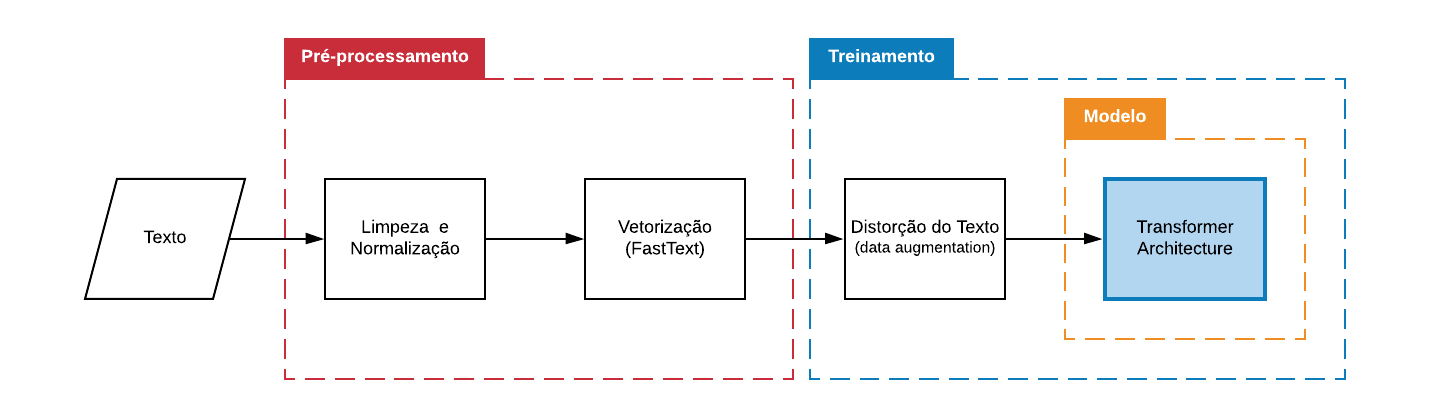
\includegraphics[width=\textwidth]{artigo/recursos/imagens/modelo_macro_texto.png}
	\end{center}
	\legend{Fonte: Elaborado pelo Autor}
\end{figure}

O texto antes do treinamento por \textbf{limpeza e normalização}, \textbf{vetorização} e durante o treinamento o texto recebe \textbf{distorções} em toda interação e então passa pela arquitetura \textbf{Transformer}.

\subsection{LIMPEZA E NORMALIZAÇÃO}

Todo o texto utilizado passa por uma função de limpeza e normalização a fim de remover a maior quantidade de inconsistências e simplificar seu formato. A função de normalização pode ser encontrada no \autoref{chap:funcao_normalizacao_texto}.

\subsection{VETORIZAÇÃO}

A representação do texto de forma vetorial para que possa ser utilizada nos modelos, precisam ser simples e que contenham em si as informações sobre o significado das palavras.

Para o nosso caso, obtivemos melhores resultados usando o \textbf{FasText} proposto no artigo \cite{fasttext}. Esse método de representação vetorial é interessante, pois diferente do \textbf{CBOW} e \textbf{SKIP-GRAM} introduzidos no artigo \cite{mikolov}, o FastText é capaz de representar palavras que não foram vistas durante o treinamento o que é uma grande vantagem no nosso contexto pois muitos termos seguem um padrão de formação, como no exemplo à seguir, onde apenas muda um carácter no modelo do smartphone.

\begin{itemize}
\item Smartphone Samsung Galaxy \textbf{S10} ...
\item Smartphone Samsung Galaxy \textbf{S10e} ...
\item Smartphone Samsung Galaxy \textbf{S10+} ...
\end{itemize}

\subsubsection{REPRESENTAÇÃO DAS PALAVRAS}

As palavras são representadas pela soma da representação vetorial de seus \textit{n-grams} mais um termo especial que é a própria palavra se ela estiver presente no dicionário. Caso a palavra não esteja presente no dicionário, então ela só será representada somente pela soma de seus \textit{n-grams}.

Note que na primeira parte da \autoref{fasttext_representacao_das_palavras_ngram} a palavra “água” aparecer como um termo especial, enquanto na segunda parte o termo especial não aparece, dando a ideia de que não esta presente no dicionário, portanto a representação da palavra será feita somente pelos seus \textit{n-grams}.

\begin{figure}[]
	\caption{\label{fasttext_representacao_das_palavras_ngram} Representação das palavras pelos seus n-grams}
	\begin{center}
	    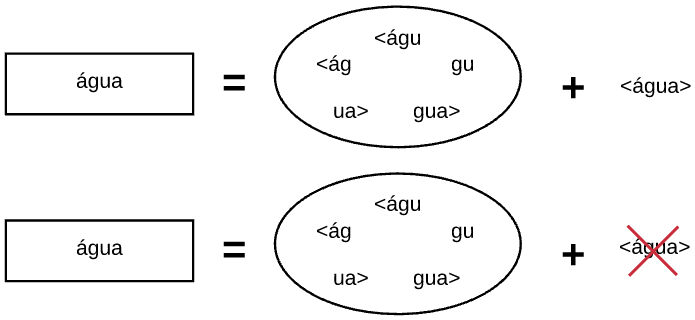
\includegraphics[scale=0.5]{artigo/recursos/imagens/fasttext_representacao_das_palavras_ngram.png}
	\end{center}
	\legend{Fonte: Elaborado pelo Autor}
\end{figure}

Vale notar que o FastText já possui diversos modelos pré-treinados em várias línguas e podem ser encontradas no seu site \href{https://fasttext.cc/docs/en/english-vectors.html}{FastText Models}.

No entanto, para maximizar a performance do modelo, foi necessário fazer um treinamento especializado com os dados do e-commerce. Para mais detalhes, veja no \autoref{chap:fasttext_modelo_pretreinado}.

\subsubsection{MODELO FASTTEXT}

O modelo do FastText é uma variação do \textbf{skip-gram} introduzido no \cite{mikolov}que tem como objetivo prever as palavras ao seu redor de forma a maximizar as suas probabilidades. Um exemplo dessa ideia pode ser visto na \autoref{skip_gram_model}.

\begin{figure}[]
	\caption{\label{skip_gram_model} SKIP-GRAM Model}
	\begin{center}
	    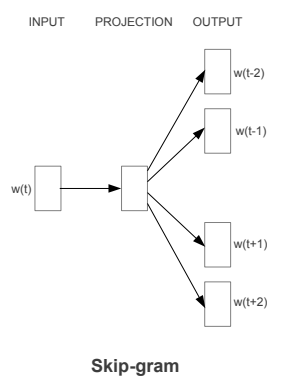
\includegraphics[scale=0.5]{artigo/recursos/imagens/skip_gram_model.png}
	\end{center}
	\legend{Fonte: Disponível em \cite{mikolov}}
\end{figure}

A definição do modelo do skip-gram é dado pela seguinte função:

\begin{center}\large
    $\sum_{t=1}^{T} = \left [ \sum_{c \in C_t} l(s(w_t, w_c))) + \sum_{n \in N_{t,c}} l(-s(w_t, n)) \right ]$
\end{center}

Tal que $w_t$ são as palavras em volta e $w_c$ é o contexto e $n$ são amostras randômicas negativas e $l$ é a \textbf{função logística de custo} (logistic loss function).

\begin{center}\large
    $l(x) = log(1 + e^{-x})$
\end{center}

O modelo de "subword" (sub-palavra) é dado pela função:

\begin{center}\large
    $s(w, c) = \sum_{g \in G_w} z_{g}^{T} v_c$
\end{center}

Onde $G$ é o tamanho do dicionário de \textit{n-grams} e dado um $w$ (palavra) as suas partes estarão contidas em G, $G_w \subset {1, ..., G}$. A representação vetorial de cada n-gram é dado por $z_g$ e a representação da palavra em si, será o seu somatório.

\subsection{DISTORÇÃO DO TEXTO}
\label{distorcao_de_texto_chap}

Para tornar o treinamento mais genérico possível e com maior variabilidade de dados, são utilizados dois tipos de distorção no texto (data augmentation), sendo a primeira de remover palavras e a segunda inverter a ordem de palavras de forma randômica.

A hipótese para esta distorção parte do principio que ao remover e trocar de posição um subconjunto pequeno de palavras não corrompe o entendimento do produto. As funções que implementam essa funcionalidade estão disponíveis no \autoref{chap:funcao_distorcao_texto}.

\begin{figure}[]
	\caption{\label{distorcao_de_texto} Visualização da Distorção de Texto}
	\begin{center}
	    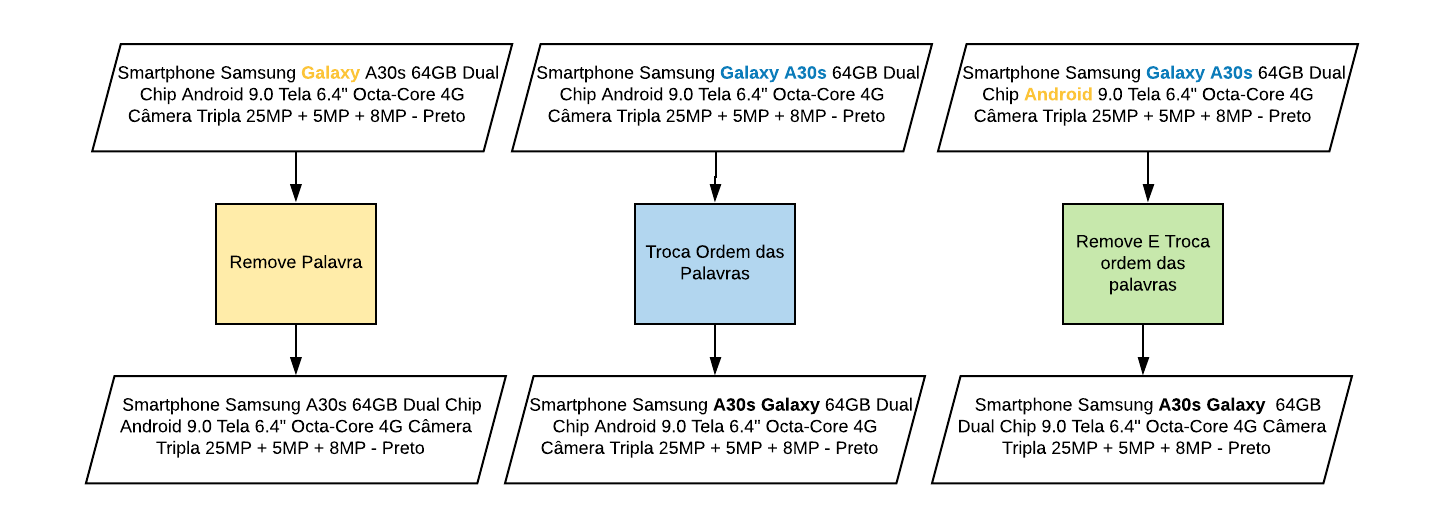
\includegraphics[width=\textwidth]{artigo/recursos/imagens/distorcao_de_texto.png}
	\end{center}
	\legend{Fonte: Elaborado pelo Autor}
\end{figure}

\subsection{ARQUITETURA TRANSFORMER}

É utilizado a arquitetura \textbf{"Transformer"} proposta no artigo \cite{transformer} que é responsável pela a extração dos atributos dos textos.

\begin{figure}[]
	\caption{\label{transformer_architecture} Arquitetura Transformer}
	\begin{center}
	    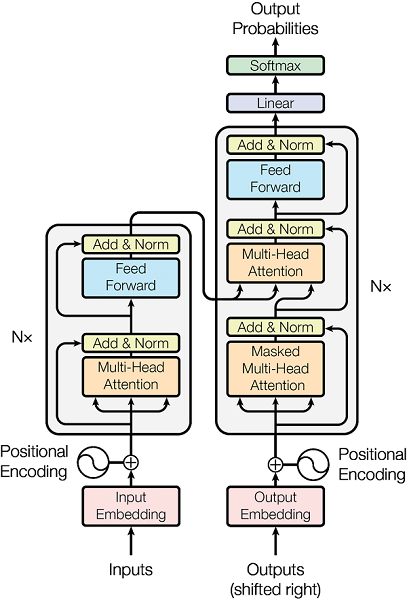
\includegraphics[scale=0.5]{artigo/recursos/imagens/transformer_architecture.png}
	\end{center}
	\legend{Fonte: Disponível em \cite{transformer}}
\end{figure}

A arquitetura é constituída de dois principais blocos. O Codificador (Encoder) e o Decodificador (Decoder) para fazer a tradução de textos. Dentro do nosso contexto, que envolve a categorização de produtos, utilizamos apenas o bloco \textbf{Codificador}. A ilustração desse bloco pode ser visto na \autoref{transformer_bloco_codificador}.

\begin{figure}[]
	\caption{\label{transformer_bloco_codificador} Bloco Codificador da Arquitetura Transformer}
	\begin{center}
	    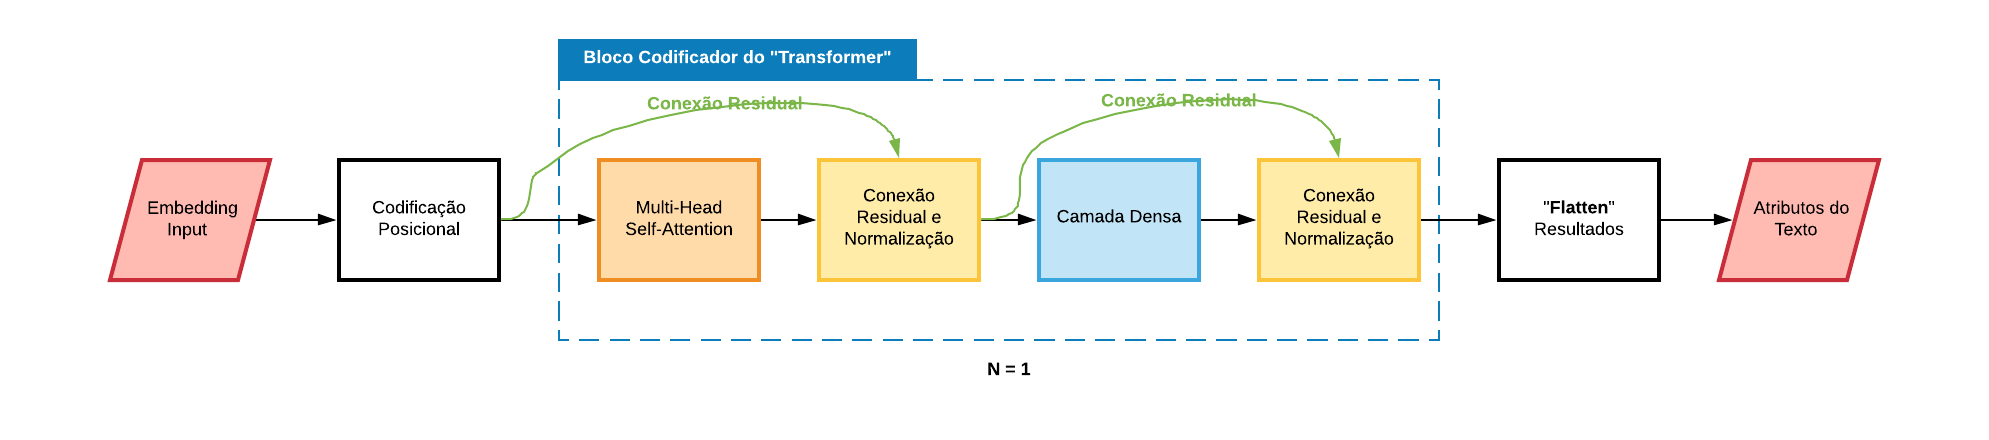
\includegraphics[scale=0.5]{artigo/recursos/imagens/transformer_bloco_codificador.png}
	\end{center}
	\legend{Fonte: Elaborado pelo Autor}
\end{figure}

\subsubsection{EMBEDDING INPUT}

O “Embedding Input” é um \textbf{$X_{b,s,d}$} é a representação do texto em formato vetorial. Esses vetores são criados à partir do modelo de FastText introduzido por \cite{fasttext} e distorcido. A distorção pode ser entendida no \autoref{distorcao_de_texto_chap}.

O tamanho da matriz é dados por \textbf{$b$} é o tamanho do lote (batch), \textbf{$s$} é o tamanho da sequência (quantidade de palavras) e \textbf{$d$} é a quantidade de dimensões do vetor das palavras.

O tamanho de \textbf{$s$} varia conforme o conjunto de dados de treinamento, e busca informar qual o tamanho adequado da quantidade máxima de palavras que será utilizado para formar as sequências removendo as discrepâncias (“outliers”) e reduzindo assim a complexidade do modelo. Essa quantidade de palavras é dada pela função:

\begin{center}
    $A = \{c_1, ..., c_n\}$ \\
    $k = \left \lceil p(n+1) / 100 \right \rceil$
\end{center}

Onde $A$ é uma sequência ordenada da quantidade de palavras por amostra do conjunto de dados de treinamento, $p$-ésimo é a parte  do conjunto de dados que estamos buscando (foi utilizado o valor de $p$ igual à 99,7) e $n$ é o tamanho do conjunto de dados, ambos os valores são calculados à partir do conjunto de dados de treinamento. O resultado $k$ é o posição de $A$ que representa a quantidade de palavras que será utilizada.

\subsubsection{CODIFICAÇÃO POSICIONAL}

Nesta etapa, o objetivo é adicionar a informação de posição nas sequênclatex colchetesias. Isso se faz necessário pois o modelo não possui consciência do que é posição, diferente de uma \textbf{Rede Neural Recorrente}. A função para a codificação das sentenças se dá por:

\begin{center}
$PE(pos, i) = \begin{cases}
sin(pos / 10000^{2i/d}), & i \in [0, i // 2) \\
cos(pos / 10000^{2i/d}), & i \in [i // 2, i]
\end{cases}$
\end{center}

Onde $d$ é o tamanho do vetor dos palavras e $i$ é um vetor de tamanho $d$ que representa a posição de cada atributo do vetor de palavra.

\begin{center}
    $i = \begin{bmatrix} 0, 1, ..., d-1 \end{bmatrix}$
\end{center}

Enquanto $pos_{b,s}$ é uma matriz onde $b$ é o tamanho do lote e $s$ é a quantidade de palavras na sequência.

\begin{center}
    $pos_{b, s} = \begin{bmatrix}
    0 & 1 & 2 & ... & s-1 \\
    0 & 1 & 2 & ... & s-1 \\
    ... \\
    0 & 1 & 2 & ... & s-1
    \end{bmatrix}$
\end{center}

A implementação do \textbf{Codificação Posicional} pode ser visto no \autoref{chap:transformer_codificao_posicional}.


\subsubsection{ATTENTION MECHANISM}

O \textbf{Attention Mechanism} (Mecanismo de Atenção em tradução direta) introduzido por \cite{attention} é um dois conceitos mais interessantes no momento. A ideia consiste em \textbf{"prestar atenção"} em uma parte da informação em detrimento de tudo. Uma visualização desse mecanismo pode ser vista na \autoref{attention_example}.

\begin{figure}[h]
	\caption{\label{attention_example} Exemplo de utilização do mecanismo de atenção em uma sequência}
	\begin{center}
	    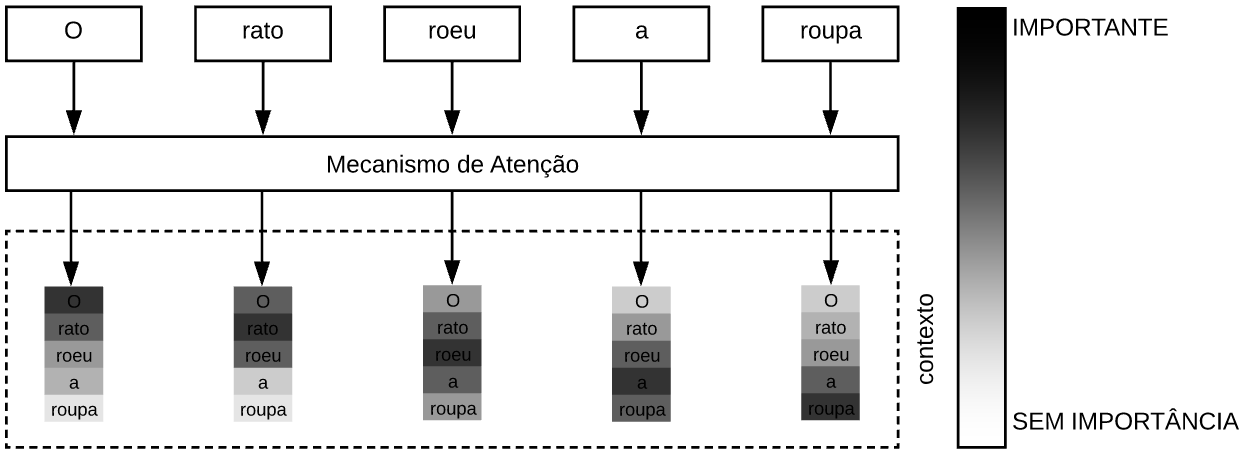
\includegraphics[width=\textwidth]{artigo/recursos/imagens/attention_example.png}
	\end{center}
	\legend{Fonte: Elaborado pelo Autor}
\end{figure}

Dado uma sequencia de palavras $h_x$ ($h_1, .., h_T$) é necessário computar um contexto $c_i$ para cada $h_i$. Criando assim um contexto individual por palavras que pode ser dado pela função de soma ponderada como pode ser visto na função à baixo.

\begin{center}\large
    $c_i = \sum_{j=1}^{T_x} \alpha_{ij} h_j$
\end{center}

Os pesos $\alpha_{ij}$ da soma ponderada é dado pela função \textbf{softmax}

\begin{center}\large
    $\alpha_{ij} = \frac{exp(e_{ij})}{\sum_{k=1}^{T_x} exp(e_{ik})}$
\end{center}

onde $e_{ij}$ é a função de alinhamento do modelo que diz o quão importante é $h_j$ é para a saída $s_{i-1}$.

\begin{center}\large
    $e_{ij} = a(s_i-1, h_j)$
\end{center}

\subsubsection{MULTI-HEAD ATTENTION}

\textbf{Muli-Head Attention} (Atenção de Múltiplas Cabeças em tradução direta) introduzido por \cite{transformer} consiste em utilizar o \textbf{Attention Mechanism} proposto no artigo \cite{attention} em projeções à partir da sequencia de entrada. Essas projeções são feitas re-organizando o os vetores das palavras $d_{model}$ em $h$ projeções.

\begin{figure}[h]
	\caption{\label{attention_muilt_head} Scaled Dot-Product Attention e Muilt-Head Attention}
	\begin{center}
	    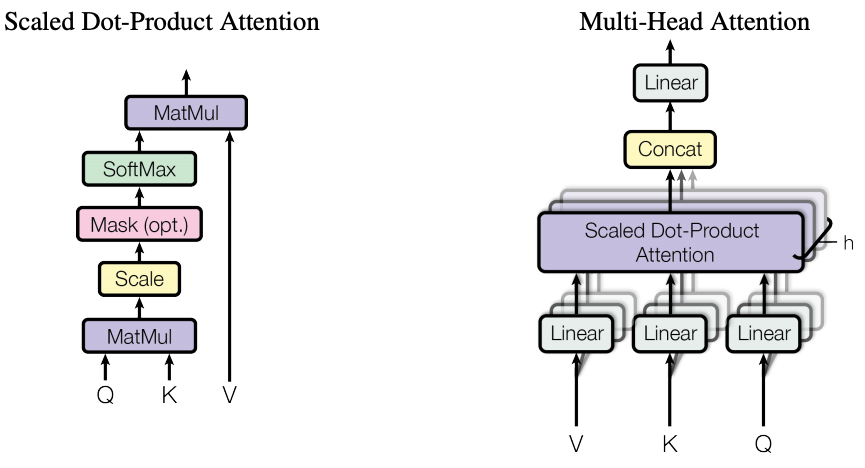
\includegraphics[width=\textwidth]{artigo/recursos/imagens/attention_muilt_head.png}
	\end{center}
	\legend{Fonte: \cite{transformer}}
\end{figure}

\textbf{Scalled Dot-Product Attention Mechanism}

Na arquitetura Transformer, é implementado uma variação do \textbf{Attention Mechanism} introduzido por \cite{attention} que é a escala do produto entre a \textbf{Query} e a \textbf{Key}.

\begin{center}
    $Attention(Q, K, V) = \frac{Q * K}{sqrt(d_{model})}*V $
\end{center}

\section{IMAGEM}

Para a extração dos atributos das imagens é utilizado o modelo da ResNet proposto no artigo \cite{resnet} além das imagens passarem por distorções em cada nova interação. O formato da estada das imagens é no formato \textbf{RGB 64x64x3}.

\begin{figure}[]
	\caption{\label{modelo_imagem_macro} Arquitetura do modelo de Imagem}
	\begin{center}
	    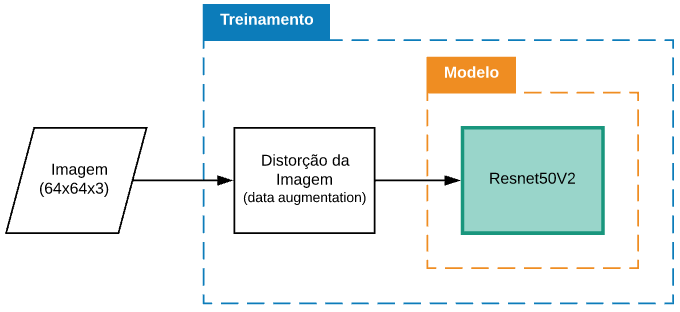
\includegraphics[scale=0.5]{artigo/recursos/imagens/modelo_imagem_macro.png}
	\end{center}
	\legend{Fonte: Elaborado pelo Autor}
\end{figure}


\subsection{DISTORÇÃO DAS IMAGENS}

Assim como foi feito nos textos, também é feito a distorção (data augmentation) nas imagens para tornar o treinamento melhor e mais genérico, pois toda vez que uma imagem passa pela rede, é como se fosse uma nova imagem. Para atingir esse objetivo é empregado diversas modificações nas imagens como pode ser visto no exemplo na \autoref{imagem_distorcao} e no \autoref{chap:funcao_distorcao_imagem} pode ser encontrado a implementação.

\begin{figure}[htb]
	\caption{\label{imagem_distorcao} Distorção de Imagens}
	\begin{center}
	    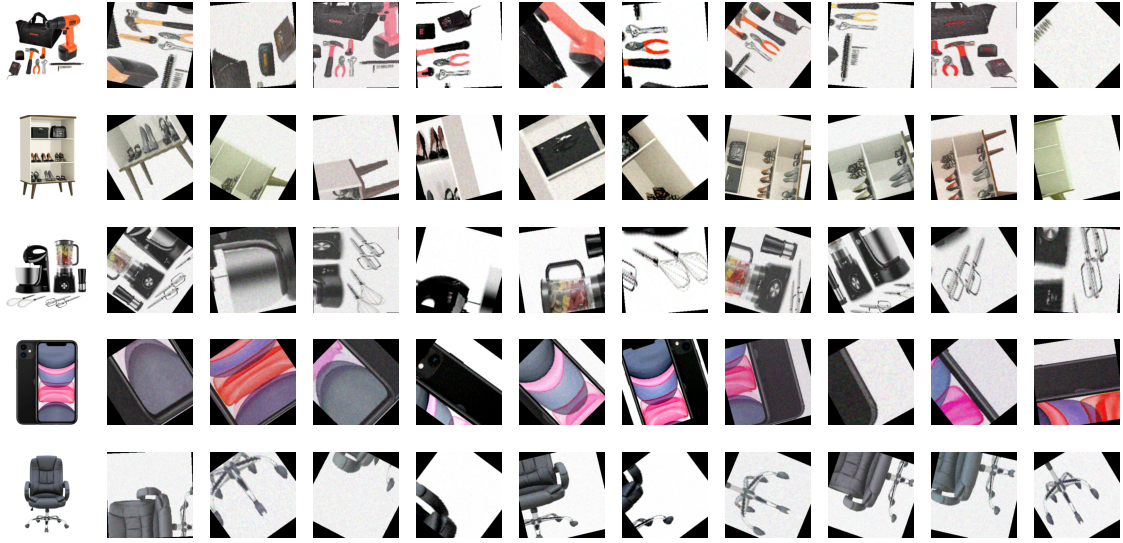
\includegraphics[width=\textwidth]{artigo/recursos/imagens/imagem_distorcao.png}
	\end{center}
	\legend{Fonte: Elaborado pelo Autor}
\end{figure}

\subsection{ARQUITETURA RESNET}

Para a extração das características das imagens é utilizado o modelo \textbf{ResNet} introduzido no \cite{resnet}, onde propõe a utilização do \textbf{bloco residual} de tal forma que previna o \textbf{vanishing e exploding} gradientes em redes neurais muito profundas. O bloco residual pode ser visto na \autoref{residual_block}.

\begin{figure}[htb]
	\caption{\label{residual_block} Bloco Residual}
	\begin{center}
	    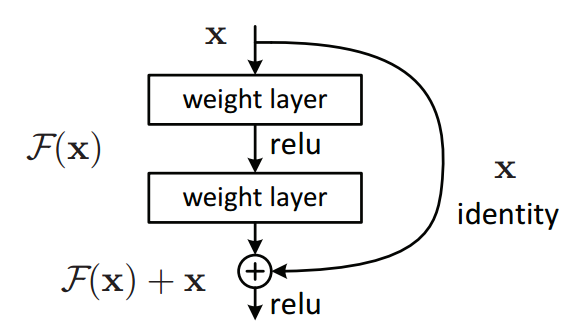
\includegraphics[scale=0.4]{artigo/recursos/imagens/residual_block.png}
	\end{center}
	\legend{Fonte: \cite{resnet}}
\end{figure}

Vale notar que o bloco residual não aumenta a complexidade da rede, pois a sua função é combinar o bloco interno com a própria identidade, também chamado de \textbf{"shortcut connections"}.

\begin{center}
    $F(x) + x$
\end{center}

Para este trabalho, utilizamos como base a \textbf{ResNet} com cinquenta (50) camadas pré-treinadas. Sabemos que existem muitas outras arquiteturas melhores, no entanto, todas trazem consigo maior complexidade, traduzindo para a realidade, um maior tempo de treinamento. Com essa versão das ResNet conseguimos obter excelentes resultados.

\begin{figure}[htb]
	\caption{\label{resnet_convs} Arquiteturas dos blocos convolucionais da ResNet}
	\begin{center}
	    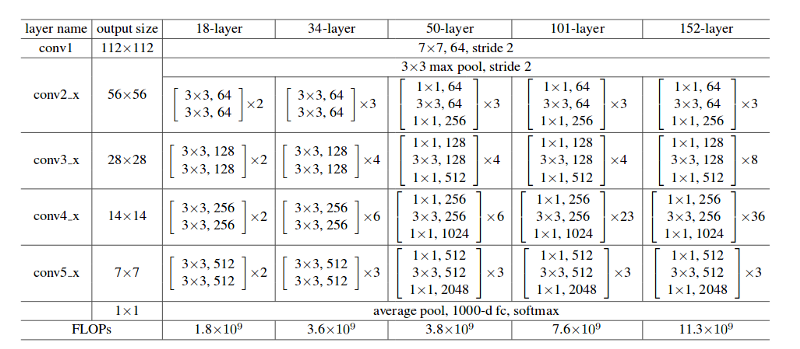
\includegraphics[width=\textwidth]{artigo/recursos/imagens/resnet_convs.png}
	\end{center}
	\legend{Fonte: \cite{resnet}}
\end{figure}


\section{CONJUNTO DE DADOS}

Como não há uma possibilidade no momento de criar um conjunto de dados anotados manualmente, utilizamos os produtos já classificados previamente. Com isso, o conjunto de dados é separado em três partes:


\begin{itemize}
\item Conjunto de dados de treinamento (inclui técnica de oversampling e undersampling)
\item Conjunto de dados de validação (utilizado para acompanhar a performance do modelo durante o treinamento é usado na cláusula de parada)
\item Conjunto de dados de teste (utilizado para criar o relatório final)
\end{itemize}

\subsection{SELEÇÃO DO CONJUNTO DE DADOS}

Para tentar criar um conjunto de dados razoável precisamos aplicar algumas técnicas para limpeza e normalização dos dados:

\begin{itemize}
\item Para tentar reduzir o ruído no conjunto de dados, é utilizado um modelo de auxiliar capaz de identificar possíveis produtos mal categorizados;
\item Quanto os produtos de uma subfamília possuem quantidade menor ou igual à 3, essas subfamílias são removidas pois não possuem dados o suficiente para treinar, validar e testar;
\item Uma vez o conjunto de dados selecionado, é feito a separação dos dados de treinamento, validação e teste. Onde 90\% dos dados são para treinamento, 5\% para validação e 5\% para teste. Os dados de treinamento passam ainda por \textbf{oversampling} e \textbf{undersampling};
\end{itemize}

\textbf{Undersampling}

Para as subfamílias com muitos produtos, é feito o \textbf{undersampling} definindo por

\begin{center}
    $mean + 2 * std$
\end{center}

\textbf{Oversampling}

Enquanto o oversampling é utilizado para famílias com menos de 30 exemplos. É feito a replicação de alguns desses meses exemplos para ter um total de 30 exemplos no final.

\section{OTIMIZAÇÃO E FUNÇÃO DE ERRO}

Para a otimização e erro é utilizado o SGD e o Focal Loss que serão descritos à seguir.

\subsection{OTIMIZADOR}

O otimizador utilizado é o \textbf{Stochastic Gradient Descent} (SGD) com \textbf{Momentum} e \textbf{Nesterov} onde obtemos melhores resultados. Usando um \textbf{Learning Rate} inicial de 0,01 com um \textbf{Learning Rate Scheduler Exponencial} sendo acionado após a 10ª época.

\subsection{FUNÇÃO DE ERRO (LOSS FUNCTION)}

Devido ao desbalanceado dados nas classes, problema que se agrava conforme a especificidade da categoria aumenta, buscamos na literatura formas para mitigar este problema, além da utilização de oversampling e undersampling passamos à utilizar também uma função de erro para ajudar neste processo.

No artigo \textbf{Focal Loss for Dense Object Detection} introduzido por \cite{local_loss} implementa uma variação do \textbf{Cross Entropy} focada em classes extremamente desbalanceadas. A implementação pode ser visto no \autoref{chap:focal_loss}.

\begin{center}
    $FL(p) = -\alpha( (1 - p) ^ l) * log(p)$
\end{center}